%% LyX 2.3.4.2 created this file.  For more info, see http://www.lyx.org/.
%% Do not edit unless you really know what you are doing.
\documentclass[english,american]{IEEEtran}
\usepackage[T1]{fontenc}
\usepackage[latin9]{inputenc}
\usepackage[letterpaper]{geometry}
\geometry{verbose,tmargin=2cm,bmargin=2.2cm,lmargin=2.2cm,rmargin=2.2cm}
\usepackage{color}
\usepackage{babel}
\usepackage{array}
\usepackage{calc}
\usepackage{amsmath}
\usepackage{amssymb}
\usepackage{graphicx}
\usepackage{wasysym}
\PassOptionsToPackage{normalem}{ulem}
\usepackage{ulem}
\usepackage[unicode=true]
 {hyperref}

\makeatletter

%%%%%%%%%%%%%%%%%%%%%%%%%%%%%% LyX specific LaTeX commands.
%% Because html converters don't know tabularnewline
\providecommand{\tabularnewline}{\\}

%%%%%%%%%%%%%%%%%%%%%%%%%%%%%% User specified LaTeX commands.
%\usepackage{lmodern}

\usepackage[T1]{fontenc}



\usepackage{courier}
\usepackage{array}

\usepackage{color}

\usepackage{upquote}

\usepackage{xcolor}

\usepackage{listings}
\usepackage[most]{tcolorbox}

\usepackage{caption}
\usepackage{graphics}
\usepackage{placeins}
\usepackage{graphicx, epstopdf}
\usepackage[framed, numbered]{matlab-prettifier}
\usepackage{colortbl}

\definecolor{celadon}{rgb}{0.67, 0.88, 0.69}
\definecolor{hellgelb}{rgb}{1,1,0.85} 
\definecolor{colKeys}{rgb}{0,0,1} 
\definecolor{colIdentifier}{rgb}{0,0,0} 
\definecolor{colComments}{rgb}{0,0.5,0} 
\definecolor{colString}{rgb}{0.81,0.12,0.95}
 \lstset{%     
 language=Matlab,%    
  float=hbp,%     
 basicstyle=\footnotesize\ttfamily,%    
  identifierstyle=\color{colIdentifier},%    
  keywordstyle=\color{colKeys},%    
  stringstyle=\color{colString},%     
 commentstyle=\itshape\color{colComments},%     
 columns=fixed,      tabsize=4,%    
  frame=single,%     
 framerule=1pt,    
  extendedchars=true,%  
    showspaces=false,%     
 showstringspaces=false,%      
numbers=left,%      
numberstyle=\tiny\ttfamily,%    
  numbersep=1em,%    
  breaklines=true,%  
    breakindent=10pt,% 
     backgroundcolor=\color{hellgelb},%  
    breakautoindent=true,%   
   captionpos=t,%   
   xleftmargin=1em,%   
   xrightmargin=\fboxsep%
}

\lstset{style=Matlab-editor, basicstyle=\ttfamily\scriptsize,captionpos=b}

\DeclareFixedFont{\ttb}{T1}{txtt}{bx}{n}{12} % for bold
\DeclareFixedFont{\ttm}{T1}{txtt}{m}{n}{12}  % for normal

\usepackage{color}
\definecolor{deepblue}{rgb}{0,0,1}
\definecolor{deepred}{rgb}{0.6,0,0}
\definecolor{deepgreen}{rgb}{0,0.5,0}

\lstset { %
language=Python,
%basicstyle=\ttm,
belowcaptionskip=1\baselineskip,
breaklines=true,
otherkeywords={self, for, enumerate},             % Add keywords here
keywordstyle=\color{deepblue},
emph={train, test ,__init__},          % Custom highlighting
emphstyle=\bfseries\color{deepred},    % Custom highlighting style
stringstyle=\color{deepgreen},
commentstyle=\itshape\color{deepgreen},
frame=tb,                         % Any extra options here
showstringspaces=false            % 
}

\hypersetup{
  colorlinks,
  citecolor=black,
  linkcolor=red,
  urlcolor=blue}

\usepackage{arydshln}
%https://tex.stackexchange.com/questions/50747/options-for-appearance-of-links-in-hyperref
%\usepackage{hyperref}
%\hypersetup{
%    colorlinks = false,
%    linkbordercolor = {white}
%}

%https://tex.stackexchange.com/questions/439768/put-reference-above-equal-sign-and-refer-to-it/439785

\newcounter{relctr} %% <- counter for relations
%\everydisplay\expandafter{\the\everydisplay\setcounter{relctr}{0}} %% <- reset every eq
\renewcommand*\therelctr{\alph{relctr}} %% <- label format

\newcommand\labelrel[2]{%
  \begingroup
    \refstepcounter{relctr}%
    \stackrel{\textnormal{(\alph{relctr})}}{\mathstrut{#1}}%
    \originallabel{#2}%
  \endgroup
}
\AtBeginDocument{\let\originallabel\label} %% <- store original definition

\@ifundefined{showcaptionsetup}{}{%
 \PassOptionsToPackage{caption=false}{subfig}}
\usepackage{subfig}
\makeatother

\begin{document}
\title{MINVO Basis: Finding Simplexes with Minimum Volume Enclosing Polynomial
Curves}
\author{Jesus Tordesillas, and Jonathan P. How\thanks{The authors are with the Aerospace Controls Laboratory, MIT, 77 Massachusetts
Ave., Cambridge, MA, USA \tt{\{jtorde, jhow\}}@mit.edu}}

\maketitle
\renewcommand{\lstlistingname}{Script}

\begin{abstract}
Outer polyhedral representations of a given polynomial curve are extensively
exploited in computer graphics rendering, computer games, path planning
for robots and finite element simulations. B�zier curves (which use
the Bernstein basis) or B-Splines are a very common choice for this,
since their partition-of-unity property guarantees that each interval
of the curve is contained inside the convex hull of its control points.
However, the convex hull provided by these bases is not the one with
smallest volume, causing therefore great conservatism in all the applications
mentioned before. This paper derives and presents the MINVO basis,
a polynomial basis that generates the smallest $n$-simplex that encloses
any given $n$-th order polynomial curve. We show that the MINVO basis
is able to obtain a volume that is $2.36$ times smaller when $n=3$,
and $903$ times smaller when $n=7$. Moreover, we show that the MINVO
basis also finds the polynomial curve with biggest convex hull enclosed
in a given simplex. Global optimality is discussed and proven for
some $n$ using Branch and Bound, Sum-Of-Squares (SOS) Programming
and moment relaxations. 
\end{abstract}


\section*{Supplementary material}

The code used for this paper is available in the following link: \textcolor{red}{Delete
this for the anonymous review}

\vspace{0.2cm}

{\tiny{}\href{https://www.google.com}{https://www.google.com}}{\tiny\par}

\section{Introduction \label{sec:Introduction}}

\begin{figure}
\subfloat[For any given $3^{rd}$-degree polynomial given, the MINVO basis finds
an enclosing simplex that is 2.36 and 254.9 times smaller than the
one found by the Bernstein or B-Spline bases respectively. \label{fig:Comparison3d_poly_given} ]{\begin{centering}
\includegraphics[width=1\columnwidth]{src/imgs/comparisonBSBeMV}
\par\end{centering}
}

\subfloat[For any given $3$-simplex, the MINVO basis finds a polynomial curve
inscribed in the simplex, and whose convex hull is 2.36 and 254.9
times bigger than the one found by the Bernstein or B-Spline bases
respectively. \label{fig:Comparison3d_simplex_given}]{\begin{centering}
\includegraphics[width=1\columnwidth]{src/imgs/comparison3d_simplex_given_compressed}
\par\end{centering}
}\caption{Comparison between the MINVO, Bernstein and B-Spline bases for $n=3$.
MINVO obtains globally optimal results for $n=3$. \label{fig:Comparison3d}}
\end{figure}

B�zier and B-Spline curves are extensively used in many different
applications, which include computer aided design (\cite{dimas19993d,de1999visualization,autodeskInventor,autodeskAutocad,autodeskMaya}),
simulations and animations (\cite{bargteil2014animation,roth1998bernstein}),
and robotics (\cite{park1995zier,faraway2007modelling,vskrjanc2010optimal,jolly2009bezier,tordesillas2019faster,preiss2017trajectory,sahingoz2014generation}),
just to mention some. The ability to approximate the space occupied
by a given polynomial curve with a polyhedron is crucial for many
of these applications, specially those that need to check the intersection
between two objects in real time. For instance, many path planning
algorithms that use B�zier curves can easily ensure safety by ensuring
that the control points of the trajectory are inside the sequence
of overlapping polyhedra that define the free space (see \cite{tordesillas2019faster,preiss2017trajectory,sahingoz2014generation}
for instance). This allows to impose a finite number of constraints
only on the vertexes of this outer polyhedral representation of the
interval, instead of infinite number of constraints over all the points
of the interval of the polynomial. Moreover, this convex hull property
of B�zier curves can also be exploited to compute curve intersections,
perform ray tracing or to compute minimum distances between convex
shapes \cite{efremov2005robust,sederberg1990curve,schulz2009bezier,gilbert1988fast,cichella2017optimal}.
Other applications that benefit from having a polyhedral outer approximation
of a curve are envelope approximations in optimization \cite{bmibnb2020}
and control for dynamical systems \cite{kuti2014minimal}. These polyhedral
outer approximations could also be potentially applied to certify
adversarial robustness in neural networks (\cite{everett2020certified,wong2018provable})
for neural networks that use polynomials as an input \cite{zhao2019machine}. 

While having some other useful properties, neither the Bernstein basis
(polynomial basis used by the B�zier curves) nor the B-Spline basis
generate the smallest simplex that encloses a given interval of the
curve. This directly translates into an unnecessary conservatism in
many of these mentioned applications. The goal of this paper is to
obtain a polynomial basis that can be used to generate the simplex
with minimum volume that encloses a polynomial curve. 

The contributions of this paper are summarized as follows:
\begin{itemize}
\item Formulation of the optimization problem that solves, without loss
of generality, for the smallest $n$-simplex that encloses \textbf{any}
given polynomial curve. We show that this problem is also equivalent
to find the polynomial curve whose convex hull has maximum volume,
while being enclosed in \textbf{any} given simplex. A more tractable
formulation by imposing a specific structure in the polynomials is
also proposed. 
\item We derive the results for $n=1,2,3,4,5,6$ and $7$, obtaining simplexes
that, for $n=3$, are $2.36$ and $254.9$ times smaller than the
ones obtained using the Bernstein or B-Spline bases. For $n=7$, the
simplexes obtained are 902.7 and $2.997\cdot10^{21}$ times smaller
than the Bernstein or B-Spline bases. 
\item Global optimality is proven for $n=1,2,3$ (for both the more general
and the more tractable one) using branch and bound, moment relaxations
and SOS. 
\end{itemize}

\section{Related work}

The work by Gary Herron \cite{herron1989polynomial} attempted to
solve this exact problem for $n=2$ and $3$ by imposing a specific
structure in the form for the polynomials of the basis, and then solving
the associated nonconvex optimization problem over the roots of those
polynomials. For this specific structure of the polynomials, a global
minimizer was found for $n=2$, and local minimizer was found for
$n=3$. Similarly, in the results of \cite{kuti2014minimal}, Kuti
et al. use the algorithm proposed in \cite{li2008minimum} to obain
a minimal simplex that encloses a specific $2^{nd}$order polynomial
curve. However, it requires running the algorithm for different curves,
no global optimality is shown, and only $n=2$ was analyzed. Our work
presented in this paper goes further, and using SOS programming, it
first proposes the most general formulation that does not impose any
specific structure in the form of the polynomials (apart from the
necesary condition of being SOS), proving global and local optimality
for some $n$. Then, by imposing a structure in the polynomials, we
are able to able to find global optima for $n=1,2,3$ and local optima
$n=4,5,6,7$.

Some works have focused on the properties of the smallest $n$-simplex
that encloses a given generic convex body. Klee showed in \cite{klee1986facet}
that any locally optimal simplex (with respect to its volume) that
encloses a convex body must be a centroidal simplex (i.e. the centroid
of its facets must touch to the convex body). Applied to a curve $\boldsymbol{p}(t)$,
this would mean tha the centroid of its facets must belong to $\text{conv}\left(\boldsymbol{p}(t)\right)$.
This gives a necessary (but not sufficient) condition of local optimality.
Bounds for the volume of the smallest $n$-simplex that encloses a
given convex body have also been found (\cite{kanazawa2014minimal,galicer2019minimal}). 

When the convex body is a polyhedron (or equivalently the convex hull
of a finite sets of points), \cite{vegter1993finding} classifies
the possible minimal circumscribing simplexes, and this classification
is later on used by \cite{zhou2002algorithms}. that, exploiting also
the necessary condition found by \cite{klee1986facet}, derives a
$O(k^{4})$ algorithm that computes the smallest simplex that contains
a finite set of $k$ points. A very similar problem has also been
studied in the hyperspectral unmixing problem inside the remote sensing
community, which consists of trying to find, in a given image pixel,
the proportions (or abundances) of each macroscopic materials (endmembers)
contained in that pixel \cite{uezato2019hyperspectral}. One way to
address this problem is to find the simplex with minimum volume that
encloses a set of points (see \cite{hendrix2013minimum} for instance).
Many different iterative algorithms have been proposed towards this
end (\cite{rogge2006iterative,iordache2009unmixing,velez2003iterative}). 

The convex hull of curves has also been studied in the literature.
\cite{ranestad2009convex,sedykh1986structure,derry1956convex} studied
the boundaries of these convex hulls, while \cite{ciripoi2018computing}
focused on the patches of the convex hull of trajectories of polynomial
dynamical systems. For a parametric curve $\left[\begin{array}{cccc}
t & t^{2} & \cdots & t^{n}\end{array}\right]^{T}$ (where $t$ is in some closed interval)\cite{mazur2017convex} found
that number of points needed to represent every point in the convex
hull of this curve is $\frac{n+1}{2}$, giving therefore a tighter
bound than the ($n+1$) points found using by the Carath�odory's Theorem
\cite{caratheodory1907variabilitatsbereich,steinitz1913bedingt}.
This particular curve was also extensively analyzed by \cite{karlin1953geometry}
in the context of moment spaces and orthogonal polynomials, deriving
also the volume of the convex hull of this curve. 

\section{Preliminaries\label{sec:Notation-and-Definitions}}

\subsection{Notation and Definitions}

Unless otherwise noted, all the indexes in this paper will start at
$0$. For instance, $M_{0,3}$ is the fourth element of the first
row of the matrix $\boldsymbol{M}$. The notation used throughout
the paper is summarized in Table \ref{tab:Notation-used-in}. Let
us also introduce the two following common definitions and their respective
notations. 

\begin{table}
\begin{centering}
\begin{tabular}{|c|>{\centering}p{6cm}|}
\hline 
\textbf{Symbol} & \textbf{Meaning}\tabularnewline
\hline 
\hline 
$a$ & Scalar\tabularnewline
\hline 
$\boldsymbol{a}$ & Column vector\tabularnewline
\hline 
$\boldsymbol{A}$ & Matrix\tabularnewline
\hline 
$A$ & Set of points\tabularnewline
\hline 
$\text{conv}(\boldsymbol{p}(t))$ & Convex hull of a curve $\boldsymbol{p}(t)$\tabularnewline
\hline 
$|\boldsymbol{A}|$ & Determinant of $\boldsymbol{A}$\tabularnewline
\hline 
$\text{abs}(a)$ & Absolute value of $a$\tabularnewline
\hline 
$\propto$ & Proportional to\tabularnewline
\hline 
$\cdot_{m\times n}$ & Size of a matrix ($m$ rows $\times$ $n$ columns)\tabularnewline
\hline 
$\boldsymbol{a}\ge\boldsymbol{b}$ & Element-wise inequality\tabularnewline
\hline 
$\boldsymbol{1}$ & Column vector of ones\tabularnewline
\hline 
$\boldsymbol{0}$ & Column vector of zeros\tabularnewline
\hline 
$\boldsymbol{e}_{i}$ & $i-$th vector of the standard basis (i.e. vector with all zeros except
a $1$ in its $i-$th entry). Its size is determined by the context.\tabularnewline
\hline 
$\boldsymbol{M}_{:,c:d}$ & Matrix formed by the rows $c,c+1,...,d$ of $\boldsymbol{M}$\tabularnewline
\hline 
$\boldsymbol{t}$ & $\begin{array}{c}
\left[\begin{array}{ccc}
t^{r} & t^{r-1}\cdots & 1\end{array}\right]^{T}\\
\text{(\ensuremath{r} given by the context)}
\end{array}$\tabularnewline
\hline 
$\hat{\boldsymbol{t}}$ & $\begin{array}{c}
\left[\begin{array}{cccc}
1 & \cdots & t^{r-1} & t^{r}\end{array}\right]^{T}\\
\text{(\ensuremath{r} given by the context)}
\end{array}$\tabularnewline
\hline 
$\mathbb{S}_{+}^{m}$ & $\begin{array}{c}
\text{Positive semidefinite cone}\\
\text{(set of all symmetric positive }\\
\text{semidefinite \ensuremath{m\times m} matrices)}
\end{array}$\tabularnewline
\hline 
$\text{vol}(\cdot)$ & Volume \textcolor{red}{Lebesgue measure?}\tabularnewline
\hline 
$\text{dist}(\boldsymbol{a},\boldsymbol{\pi})$ & $\begin{array}{c}
\text{Distance between the point \ensuremath{\boldsymbol{a}} }\\
\text{and the hyperplane \ensuremath{\boldsymbol{\pi}}}
\end{array}$\tabularnewline
\hline 
$\text{Pf}(\boldsymbol{A})$ & Pfaffian of $\boldsymbol{A}$, as defined by \cite{de1955some}\tabularnewline
\hline 
$\text{MV},\text{Be},\text{BS}$ & MINVO, Bernstein and B-Spline respectively\tabularnewline
\hline 
\end{tabular}
\par\end{centering}
\caption{Notation used in this paper \label{tab:Notation-used-in}}

\end{table}

\noindent\fbox{\begin{minipage}[t]{1\columnwidth - 2\fboxsep - 2\fboxrule}%
\textbf{$n$-simplex}: Convex hull of $n+1$ points $\boldsymbol{v}_{0},...,\boldsymbol{v}_{n}\in\mathbb{R}^{n}$.
These points are \textbf{vertexes} of the simplex, and will be stacked
in the \textbf{matrix of vertexes} $\boldsymbol{V}:=\left[\begin{array}{ccc}
\boldsymbol{v}_{0} & \cdots & \boldsymbol{v}_{n}\end{array}\right]$. A simplex with $\boldsymbol{V}=\left[\begin{array}{cccc}
\boldsymbol{0} & \boldsymbol{e}_{0} & \cdots & \boldsymbol{e}_{n}\end{array}\right]$ is the \textbf{standard simplex}. The letter $S$ will denote the
simplex, while $S^{n}$ will denote the set of all possible $n$-simplexes. %
\end{minipage}}

\vspace{0.2cm}

\noindent\fbox{\begin{minipage}[t]{1\columnwidth - 2\fboxsep - 2\fboxrule}%
\textbf{Polynomial curve} \textbf{of degree} $n$ \textbf{and dimension}
$k$: Parametric curve $\boldsymbol{p}(t):=\left[\begin{array}{c}
p_{0}(t)\\
\vdots\\
p_{k-1}(t)
\end{array}\right]:=\boldsymbol{P}\boldsymbol{t}\in\mathbb{R}^{k}$, where $p_{i}(t)$ is a polynomial of degree $n$. The matrix $\boldsymbol{P}$
is the coefficient matrix, and will be denoted as $\boldsymbol{P}:=\left[\begin{array}{c}
\boldsymbol{c}_{0}^{T}\\
\vdots\\
\boldsymbol{c}_{k-1}^{T}
\end{array}\right]_{k\times(n+1)}\equiv\left[\begin{array}{ccc}
\boldsymbol{p}_{n} & \cdots & \boldsymbol{p}_{0}\end{array}\right]_{k\times(n+1)}$. In this paper, we will use the interval $t\in[-1,1]$. The subspace
that contains that interval and has smallest dimension will be denoted
as $\mathbb{R}^{m}\subseteq\mathbb{R}^{k}$. In this paper we will
work with the case $n=m=k$ (and refer to the intervals of such curves
simply as $n$-th order polynomial curves). Section \ref{sec:Embedding}
will then extend the results to the case $n=m\le k$. %
\end{minipage}}

\vspace{0.2cm}

We will use non-clamped uniform B-Splines for comparison, and refer
to them simply as B-Splines.


\subsection{Volume of the Convex Hull of a Polynomial Curve}

At several points throughout the paper, we will make use of the following
theorem, that we prove in the Appendix (Sec. \ref{sec:Appendix}):

\vspace{0.2cm}

\noindent\fcolorbox{black}{white}{\begin{minipage}[t]{1\columnwidth - 2\fboxsep - 2\fboxrule}%

\textbf{Theorem 1:} The volume of the convex hull of an $n$-th order
polynomial curve $\boldsymbol{p}(t)$, with $t\in[-1,1]$, is given
by:{\footnotesize{}
\[
\text{vol}\left(\text{conv}\left(\boldsymbol{p}(t)\right)\right)=\frac{\text{abs}\left(\left|\boldsymbol{P}_{:,0:n}\right|\right)}{n!}2^{\frac{n(n+1)}{2}}\prod_{0\le i<j\le n}\left(\frac{j-i}{j+i}\right)
\]
}{\footnotesize\par}

\textbf{Proof}: See Appendix (Sec. \ref{sec:Appendix}). \hfill $\square$

%
\end{minipage}}

\vspace{0.2cm}


\section{Problems definition}

The first problem this paper is going to investigate is the following
one:

\vspace{0.2cm}

\definecolor{problem1_color}{RGB}{255,238,213}
\definecolor{problem2_color}{RGB}{255,233,233}
\definecolor{problem3_color}{RGB}{221,243,255}
\definecolor{problem4_color}{RGB}{240,255,229}

\noindent\fcolorbox{black}{problem1_color}{\begin{minipage}[t]{1\columnwidth - 2\fboxsep - 2\fboxrule}%

\textbf{Problem 1}: Given an $n$-th order polynomial curve $\boldsymbol{p}(t)$,
find the $n$-simplex $S$ with minimum volume that contains $\boldsymbol{p}(t)$
$\forall t\in[-1,1]$. In other words:
\[
\min_{S\in S^{n}}\quad f_{1}:=\text{vol}(S)\propto\text{abs}\left(\left|\left[\begin{array}{cc}
\boldsymbol{V}^{T} & \boldsymbol{1}\end{array}\right]\right|\right)
\]

\[
\begin{array}{cc}
s.t. & \boldsymbol{p}(t)\in S\quad\forall t\in[-1,1]\end{array}
\]

%
\end{minipage}}

\vspace{0.2cm}

For $n=2$, Problem 1 tries to find the triangle with the smallest
area that contains the curve $\left[\begin{array}{cc}
x(t) & y(t)\end{array}\right]^{T}$ , where $x(t)$ and $y(t)$ are $2^{nd}$-degree polynomials. For
$n=3$, it tries to find the tetrahedron with the smallest volume
that contains the curve $\left[\begin{array}{ccc}
x(t) & y(t) & z(t)\end{array}\right]^{T}$(all $3^{rd}$-degree polynomials). As explained in \ref{sec:Notation-and-Definitions},
we will assume that the curve $\boldsymbol{p}(t)$ given satisfies
$\left|\boldsymbol{P}_{:,0:n}\right|\neq0$ (which implies that its
volume is $\neq0$). As the simplex S encloses $\boldsymbol{p}(t)$,
its volume will be $\neq0$ and therefore $\left|\left[\begin{array}{cc}
\boldsymbol{V}^{T} & \boldsymbol{1}\end{array}\right]\right|\neq0$.

The second problem of this paper is this one:

\vspace{0.2cm}

\noindent\fcolorbox{black}{problem2_color}{\begin{minipage}[t]{1\columnwidth - 2\fboxsep - 2\fboxrule}%

\textbf{Problem 2:} Given the vertexes $\boldsymbol{v}_{0},...,\boldsymbol{v}_{n}$
of an $n$-simplex $S$, find the $n$-th order polynomial curve $\boldsymbol{p}(t)$
contained in $S$, whose convex hull has maximum volume ($t\in[-1,1]$):{\footnotesize{}
\[
\min_{\boldsymbol{p}(t)}\quad f_{2}:=-\text{vol}(\text{conv}(\boldsymbol{p}(t))\propto-\text{abs}\left(\left|\boldsymbol{P}_{:,0:n}\right|\right)
\]
}{\footnotesize\par}

\[
\begin{array}{cc}
s.t. & \boldsymbol{p}(t)\in S\quad\forall t\in[-1,1]\end{array}
\]

%
\end{minipage}}

\vspace{0.2cm}

Another possible geometric interpretation of Problem 2 is that we
are trying to find the $n$-th order polynomial curve $\boldsymbol{p}(t)$
contained in $S$, whose coefficients vectors $\boldsymbol{p}_{n},...,\boldsymbol{p}_{1}$
span a parallelogram with largest volume. 

\vspace{0.2cm}

We will assume that the matrix of vertexes of the simplex $S$ given
satisfies $\left|\left[\begin{array}{cc}
\boldsymbol{V}^{T} & \boldsymbol{1}\end{array}\right]\right|\neq0$. In other words, the simplex S given is not contained in a subspace
$\mathbb{R}^{m}$, with $m<n$. Now note that the optimal solution
for this problem is guaranteed to satisfy $\left|\boldsymbol{P}_{:,0:n}\right|\neq0$
\footnote{This can be easily proven by noting that we are maximizing the absolute
value of $\left|\boldsymbol{P}_{:,0:n}\right|$, and that there exists
at least one feasible point (for example the B�zier curve whose control
points are $\{\boldsymbol{v}_{0},...,\boldsymbol{v}_{n}\}$) with
$\left|\boldsymbol{P}_{:,0:n}\right|\neq0$.}.

\section{Equivalent Formulation}

Let us now study the constraints and the objective functions of Problems
1 and 2.

\subsection{Constraints of Problem 1 and 2:\label{subsec:Constraints-of-Problem}}

Both problems share the same constraint $\boldsymbol{p}(t)\in S\quad\forall t\in[-1,1]$,
which is equivalent to $\boldsymbol{p}(t)$ being a convex combination
of the vertexes $\boldsymbol{v}_{i}$ of the simplex for $t\in[-1,1]$:
\[
\left.\begin{array}{c}
\boldsymbol{p}(t)=\sum_{i=0}^{n}\lambda_{i}(t)\boldsymbol{v}_{i}\\
\sum_{i=0}^{n}\lambda_{i}(t)=1\quad\forall t\\
\lambda_{i}(t)\ge0\quad\forall i=0,..,,n\;\;\forall t\in[-1,1]
\end{array}\right\} 
\]

The geometric interpretation of each $\lambda_{i}(t)$ is as follows.
Let us define $\boldsymbol{\pi}_{i}$ as the hyperplane that passes
through the points $\{\boldsymbol{v}_{0},\boldsymbol{v}_{1},...,\boldsymbol{v}_{n}\}\backslash\boldsymbol{v}_{i}$,
and $\boldsymbol{n}_{i}$ as the normal vector of this hyperplane
$\boldsymbol{\pi}_{i}$ that satisfies $\boldsymbol{n}_{i}^{T}\boldsymbol{p}(t)\ge0$
(i.e. pointing towards the interior of the simplex). Choosing now
a vertex $k\in\{0,...,n\}\backslash i$ we have that:

\[
\boldsymbol{p}(t)=\sum_{j=0}^{n}\lambda_{j}(t)\boldsymbol{v}_{j}=\boldsymbol{v}_{k}+\sum_{\begin{array}{c}
j=0\\
j\neq k
\end{array}}^{n}\lambda_{j}(t)\left(\boldsymbol{v}_{j}-\boldsymbol{v}_{k}\right)
\]

And therefore:
\[
\begin{array}{c}
\text{dist}\left(\boldsymbol{p}(t),\boldsymbol{\pi}_{i}\right):=\left(\boldsymbol{p}(t)-\boldsymbol{v}_{k}\right)^{T}\boldsymbol{n}=\\
\\
=\sum_{j=0}^{n-1}\lambda_{j}(t)\left(\boldsymbol{v}_{i}-\boldsymbol{v}_{k}\right)^{T}\boldsymbol{n}=\lambda_{i}(t)\;\text{dist}\left(\boldsymbol{v}_{i},\boldsymbol{\pi}_{i}\right)
\end{array}
\]

\begin{equation}
\lambda_{i}(t)=\frac{\text{dist}\left(\boldsymbol{p}(t),\boldsymbol{\pi}_{i}\right)}{\text{dist}\left(\boldsymbol{v}_{i},\boldsymbol{\pi}_{i}\right)}\label{eq:normalized_distance}
\end{equation}

Hence, each $\lambda_{i}$ represents the ratio between the distance
of the curve to the hyperplane $\boldsymbol{\pi}$ (formed by the
points $\boldsymbol{v}_{j}\;,j\neq i$) and the distance from $\boldsymbol{v}_{i}$
to that hyperplane $\boldsymbol{\pi}$ (see Fig. \ref{fig:Geometric-interpretation-of}
for the case $n=3$). \textcolor{red}{Barycentric coordinates?? }From
Eq. \ref{eq:normalized_distance} it is clear that each $\lambda_{i}(t)$
is an $n$-th degree polynomial, that we will write as $\lambda_{i}(t):=\boldsymbol{\lambda}_{i}^{T}\boldsymbol{t}$.
Matching the coefficients with $\boldsymbol{p}(t)$ we have that:

\[
\boldsymbol{P}=\boldsymbol{V}\underbrace{\left[\begin{array}{c}
\boldsymbol{\lambda}_{0}^{T}\\
\boldsymbol{\lambda}_{1}^{T}\\
\vdots\\
\boldsymbol{\lambda}_{n}^{T}
\end{array}\right]}_{:=\boldsymbol{A}}
\]

where we have also defined the $(n+1)\times(n+1)$ matrix $\boldsymbol{A}$,
whose $i$-th row contains the coefficients of the polynomial $\lambda_{i}(t)$
in decreasing order. Now note that the constraint $\sum_{i=0}^{n}\lambda_{i}(t)=1$,
can be rewritten as $\boldsymbol{A}^{T}\boldsymbol{1}=\boldsymbol{e}_{n}$
(or equivalently $\boldsymbol{e}_{n}^{T}\boldsymbol{A}^{-1}=\boldsymbol{1}^{T}\boldsymbol{A}$),
and therefore we can combine both as:
\[
\left[\begin{array}{c}
\boldsymbol{P}\\
\boldsymbol{e}_{n}^{T}
\end{array}\right]=\left[\begin{array}{c}
\boldsymbol{V}\\
\boldsymbol{1}^{T}
\end{array}\right]\boldsymbol{A}
\]

Note that the matrix $\boldsymbol{A}$ is clearly invertible: As $\text{abs}\left(\left|\begin{array}{c}
\boldsymbol{P}\\
\boldsymbol{e}_{n}^{T}
\end{array}\right|\right)=\text{abs}\left(\left|\boldsymbol{P}_{:,0:n}\right|\right)\neq0$, and $\left|\begin{array}{c}
\boldsymbol{V}\\
\boldsymbol{1}^{T}
\end{array}\right|=\left|\begin{array}{cc}
\boldsymbol{V}^{T} & \boldsymbol{1}\end{array}\right|\neq0$, we have that 
\[
\text{rank}\left(\left[\begin{array}{c}
\boldsymbol{P}\\
\boldsymbol{e}_{n}^{T}
\end{array}\right]\right)=\text{rank}\left(\left[\begin{array}{c}
\boldsymbol{V}\\
\boldsymbol{1}^{T}
\end{array}\right]\right)=n+1
\]
Therefore, and using the fact that $\text{rank}\left(\boldsymbol{B}\boldsymbol{C}\right)\le\min\left(\text{rank}\left(\boldsymbol{B}\right),\text{rank}\left(\boldsymbol{C}\right)\right)$,
we conclude that $\text{\text{rank}\ensuremath{\left(\boldsymbol{A}\right)}}=n+1$
(i.e. $\boldsymbol{A}$ has full rank). 

\begin{figure}
\begin{centering}
\includegraphics[width=1\columnwidth]{src/imgs/geom_meaning_lambdai}
\par\end{centering}
\caption{Geometric interpretation of $\lambda_{i}(t)$. Each $\lambda_{i}(t)$
represents the normalized distance between the curve $\boldsymbol{p}(t)$
and the hyperplane formed by the vertexes $\boldsymbol{v}_{i},\;i\protect\neq j$,
normalized with the distance from the vertex $\boldsymbol{v}_{i}$
to that plane (left). For a standard simplex in 3D (i.e. $\boldsymbol{V}=\left[\protect\begin{array}{cccc}
\boldsymbol{0} & \boldsymbol{e}_{0} & \boldsymbol{e}_{1} & \boldsymbol{e}_{2}\protect\end{array}\right]$) (right), the curve in red is $\boldsymbol{p}(t)=\left[\protect\begin{array}{ccc}
\lambda_{1}(t) & \lambda_{2}(t) & \lambda_{3}(t)\protect\end{array}\right]^{T}$.\label{fig:Geometric-interpretation-of}}

\vskip-2ex
\end{figure}


\subsection{Objective Function of Problem 1}

Given the previous relationships, we have that 

\[
\left|\left[\begin{array}{cc}
\boldsymbol{V}^{T} & \boldsymbol{1}\end{array}\right]\right|=\left|\boldsymbol{A}^{-T}\left[\begin{array}{c}
\boldsymbol{P}^{T}\boldsymbol{e}_{n}\end{array}\right]\right|\propto\left|\boldsymbol{A}^{-1}\right|=\frac{1}{|\boldsymbol{A}|}
\]

where we have used the fact that everything inside $\left[\begin{array}{c}
\boldsymbol{P}^{T}\boldsymbol{e}_{n}\end{array}\right]$ is given (i.e. not a decision variable of the optimization problem),
and the fact that $\left|\boldsymbol{A}\right|=\left|\boldsymbol{A}^{T}\right|$.
Therefore, we conclude that $f_{1}\propto\frac{1}{\text{abs}\left(|\boldsymbol{A}|\right)}$.
We can therefore maximize $abs(\left|\boldsymbol{A}\right|)$, or,
equivalently, minimize $-\text{abs}\left(\left|\boldsymbol{A}\right|\right)$.

\subsection{Objective Function of Problem 2}

Similar to the previous subsection, we have that

\[
\left|\boldsymbol{P}_{:,0:n}\right|=\left|\left[\begin{array}{c}
\boldsymbol{P}\\
\boldsymbol{e}_{n}^{T}
\end{array}\right]\right|=\left|\left[\begin{array}{c}
\boldsymbol{V}\\
\boldsymbol{1}^{T}
\end{array}\right]\boldsymbol{A}\right|\propto\left|\boldsymbol{A}\right|
\]

And therefore, $f_{2}\propto-\text{abs}\left(\left|\boldsymbol{A}\right|\right)$. 

\subsection{Equivalent Formulation for Problem 1 and 2}

Therefore, we can solve Problem 1 (or Problem 2 respectively) for
\textbf{any} given polynomial curve (\textbf{any} given simplex respectively)
by solving the following problem\footnote{Note that in Problem 3 the $\text{abs}(\cdot)$ is not necessary,
since any permutation of the rows of $\boldsymbol{A}$ will change
the sign of $\left|\boldsymbol{A}\right|$. We keep it simply for
consistency purposes, since later in the solutions we will show a
specific order of the rows of $\boldsymbol{A}$ for which (for some
$n$) $\left|\boldsymbol{A}\right|<0$, but that allows us to highlight
the similarities and differences between this matrix and the ones
Bernstein and B-Spline bases use. }: 

\vspace{0.2cm}

\noindent\fcolorbox{black}{problem3_color}{\begin{minipage}[t]{1\columnwidth - 2\fboxsep - 2\fboxrule}%

\textbf{Problem 3: }

\[
\min_{\boldsymbol{A}\in\mathbb{R}^{(n+1)\times(n+1)}}\quad f_{3}:=-\text{abs}\left(\left|\boldsymbol{A}\right|\right)
\]

\[
\begin{array}{cc}
s.t. & \boldsymbol{A}\boldsymbol{t}\ge\boldsymbol{0}\quad\forall t\in[-1,1]\\
 & \boldsymbol{A}^{T}\boldsymbol{1}=\boldsymbol{e}_{n}
\end{array}
\]

%
\end{minipage}}

\vspace{0.2cm}

As the objective function of Problem 3 is the determinant of a nonsymmetric
matrix $\boldsymbol{A}:=\left[\begin{array}{ccc}
\boldsymbol{\lambda}_{0} & \cdots & \boldsymbol{\lambda}_{n}\end{array}\right]^{T}$, it is clearly a nonconvex problem. For the first constraint of Problem
3, we can use the following result of Sum-Of-Squares programming,
to rewrite that constraint and leave positive semidefinite matrices
as decision variables \cite{Parrilo09}: \textcolor{red}{CHECK}
\begin{itemize}
\item If $n$ is odd, $\lambda_{i}(t)\ge0\;\;\forall t\in[-1,1]$ if and
only if
\end{itemize}
\[
\left\{ \begin{array}{c}
\lambda_{i}(t)=\hat{\boldsymbol{t}}^{T}\left((t+1)\boldsymbol{W}_{i}+(1-t)\boldsymbol{V}_{i}\right)\hat{\boldsymbol{t}}\\
\boldsymbol{W}_{i}\in\mathbb{S}_{+}^{\frac{n+1}{2}},\boldsymbol{V}_{i}\in\mathbb{S}_{+}^{\frac{n+1}{2}}
\end{array}\right.
\]

\begin{itemize}
\item If $n$ is even, $\lambda_{i}(t)\ge0\;\;\forall t\in[-1,1]$ if and
only if
\end{itemize}
\[
\left\{ \begin{array}{c}
\lambda_{i}(t)=\hat{\boldsymbol{t}}^{T}\boldsymbol{W}_{i}\hat{\boldsymbol{t}}+\hat{\boldsymbol{t}}^{T}(t+1)(1-t)\boldsymbol{V}_{i}\hat{\boldsymbol{t}}\\
\boldsymbol{W}_{i}\in\mathbb{S}_{+}^{\frac{n}{2}+1},\boldsymbol{V}_{i}\in\mathbb{S}_{+}^{\frac{n}{2}}
\end{array}\right.
\]

Note that the \emph{if and only if} condition applies because it is
a univariate polynomial \cite{Parrilo09}. We end up therefore with
a nonconvex finite-dimensional optimization problem, where the decision
variables are the positive semidefinite matrices $\boldsymbol{W}_{i}$
and $\boldsymbol{V}_{i}$, $i=0,...,n$. 

No generality has been lost in Problem 3. However, this problem easily
becomes intractable for large $n$. To make it more tractable, we
can try to reduce the number of decision variables of Problem 3 by
imposing a structure in $\lambda_{i}(t)$. As Problem 1 is trying
to minimize the volume of the simplex, we can impose that the facets
of the $n$-simplex be tangent \textcolor{red}{(vale xa nondiff points?)}
to the curve \cite{zhou2002algorithms,klee1986facet}. Using the geometric
interpretation of the $\lambda_{i}(t)$ given in subsection \ref{subsec:Constraints-of-Problem},
this means that each $\lambda_{i}(t)$ should have either real double
roots (where the curve is tangent to the plane), and/or roots at $t=\pm1$.
This translates into the formulation shown in Problem 4.

\textcolor{red}{REVISAR LAS CONSTRAINTS $\lambda_{i}(t)=\lambda_{n-i+2}(-t)$
DebajoCREO QUE ALGUN INDICE PUEDE ESTAR MAL}

\vspace{0.2cm}

\begin{figure}
\noindent\fcolorbox{black}{problem4_color}{\begin{minipage}[t]{1\columnwidth - 2\fboxsep - 2\fboxrule}%

\textbf{Problem 4:}

\[
\min_{\boldsymbol{A}\in\mathbb{R}^{(n+1)\times(n+1)}}\quad f_{4}:=-abs\left(\left|\boldsymbol{A}\right|\right)
\]

\[
s.t:
\]

\textbf{\uline{If \mbox{$n$} is odd:}}

\[
\begin{array}{c}
\lambda_{i}(t)=-b_{i}(t-1)\prod_{j=1}^{\frac{n-1}{2}}(t-t_{j})^{2}\quad i=0,2,...,n-1\\
\lambda_{i}(t)=\lambda_{n-i+2}(-t)\quad\quad\quad i=1,3,...,n\\
b_{i}\ge0\quad i=0,2,...,n-1\\
\sum_{i=0}^{n}\lambda_{i}(t)=1
\end{array}
\]

\textbf{\uline{If \mbox{$n$} is even:}} define $\mathcal{I}_{a}$
the set of odd integers $\in\left[0,\frac{n}{2}-1\right]$, and $\mathcal{I}_{b}$
the set of even integers $\in\left[0,\frac{n}{2}-1\right]$: 

\[
\begin{array}{c}
\lambda_{i}(t)=-b_{i}(t+1)(t-1)\prod_{j=1}^{\frac{n-2}{2}}(t-t_{j})^{2}\quad i\in\mathcal{I}_{a}\\
\lambda_{i}(t)=b_{i}\prod_{j=1}^{\frac{n}{2}}(t-t_{j})^{2}\quad\quad\quad i\in\mathcal{I}_{b}\\
\lambda_{j}(t)=\lambda_{n-i+1}(-t)\quad\quad\quad i=\frac{n}{2}+1,...,n\\
b_{i}\ge0\quad i\le\frac{n}{2}\\
\sum_{i=0}^{n}\lambda_{i}(t)=1
\end{array}
\]

\begin{itemize}
\item If $\frac{n}{2}$ is odd ($n=2,6,10...)$:
\end{itemize}
\[
\lambda_{i}(t)=-b_{i}(t+1)(t-1)\prod_{j=1}^{\frac{n-2}{4}}(t-t_{j})^{2}(t+t_{j})^{2}\quad\quad i=\frac{n}{2}
\]

\begin{itemize}
\item If $\frac{n}{2}$ is even ($n=4,8,12...)$:
\end{itemize}
\[
\lambda_{i}(t)=b_{i}\prod_{j=1}^{\frac{n}{4}}(t-t_{j})^{2}(t+t_{j})^{2}\quad\quad i=\frac{n}{2}
\]

%
\end{minipage}}
\end{figure}

The relationship between Problems 1, 2, 3 and 4 is given in Fig. \ref{fig:relationships_problems}.
First note that the structure imposed for $\lambda_{i}(t)$ in Problem
4 guarantees that they are nonnegative for $t\in[-1,1]$. Hence the
feasible set of Problem 4 is contained in the feasible set of Problem
3, and therefore, $f_{3}^{*}\le f_{4}^{*}$ holds. The matrix $\boldsymbol{A}^{*}$
found in Problem 3 or 4 can be used to find the vertexes of the simplex
in Problem 1 (by simply using $\boldsymbol{V}^{*}=\boldsymbol{P}\left(\boldsymbol{A}^{*}\right)^{-1}$,
where $\boldsymbol{P}$ is the coefficient matrix of the polynomial
given), or to find the coefficient matrix of the polynomial in Problem
2 (by using $\boldsymbol{P}^{*}=\boldsymbol{V}\boldsymbol{A}^{*}$,
where $\boldsymbol{V}$ contains the vertexes of the simplex given).

\begin{figure}
\begin{centering}
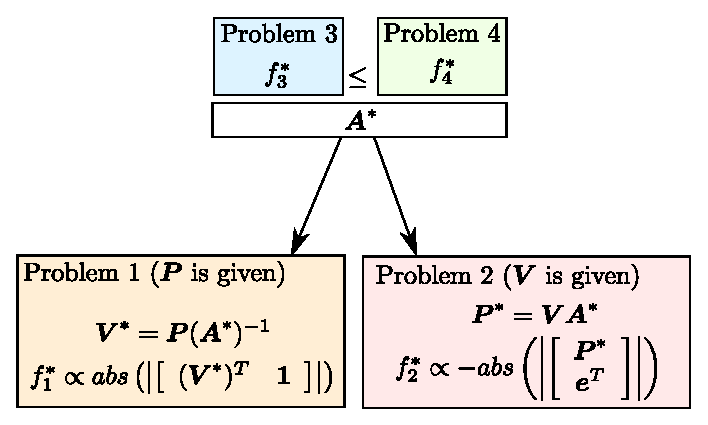
\includegraphics[width=1\columnwidth]{src/imgs/relationships_problems}
\par\end{centering}
\caption{Relationship between Problems 1, 2, 3 and 4: Problem 4 and Problem
3 have the same objective function, but the feasible set of Problem
4 is contained in the feasible set of Problem 3, and therefore $f_{3}^{*}\le f_{4}^{*}$.
Both Problem 3 and 4 generate a (potentially locally) optimal solution
$\boldsymbol{A}^{*}$, which can be applied to any polynomial curve
to find the simplex in Problem 1, or to any simplex to find the polynomial
curve in Problem 2. \label{fig:relationships_problems}}

\vskip-2ex
\end{figure}

\vspace{0.2cm}


\section{Results}

The optimization Problems 3 and 4 have been solved using the nonconvex
solvers \emph{IPOPT} \cite{wachter2006implementation} and \emph{Knitro}
\cite{byrd2006k,byrd1999interior} (for Problem 3), the \emph{fmincon}
nonconvex solver \cite{matlabOptToolbox} (for Problem 4), and the
\emph{Yalmip} interface \cite{Lofberg2004,Lofberg2009}. 

We were able to find local minima for Problem 4 for $n=1,2,3,4,5,6,7$,
and the same local minima were found in Problem 3 for $n=1,2,3,4$
(Problem 3 becomes intractable for higher $n$). The optimal matrices
$\boldsymbol{A}$ found are shown in Table \ref{tab:table_matrices},
and denoted as $\boldsymbol{A}_{\text{MV}}$. Note that any permutation
in the rows of $\boldsymbol{A}_{\text{MV}}$will not change the objective
value, since only the sign of the determinant is affected. Its determinant
$\left|\boldsymbol{A}_{\text{MV}}\right|$ is also compared with the
one of the Bernstein and B-Spline matrices (denoted as $\boldsymbol{A}_{\text{Be}}$
and $\boldsymbol{A}_{\text{BS}}$ respectively) The corresponding
plots of the MINVO basis functions are shown in Fig. \ref{fig:minvo_and_bernstein},
together with the Bernstein, B-Spline, and Lagrange bases for comparison.
The roots of each of the MINVO basis functions $\lambda_{i}(t)$ are
shown in Table \ref{tab:roots}.

One natural question to ask is whether the basis found constitutes
a global minimizer for either Problem 3 or Problem 4. To answer this,
first note that both Problem 3 and Problem 4 are polynomial optimization
problems. Therefore, we can make use of Lasserre's moment method \cite{lasserre2001},
and increase the order of the moment relaxation to find tighter lower
bounds of the original nonconvex polynomial optimization problem.
\textcolor{red}{CHECK THIS.} Using this technique, we were able to
obtain the same objective value (proving therefore global optimality)
for $n=1,2,3$ in Problem 4. For Problem 3, the moment relaxation
technique becomes instractable due to the higher number of variables
and to proble global optimality we use instead the branch-and-bound
algorithm, that proves global optimality by reducing to $0$ the gap
between the upper bounds found by a nonconvex solver, and the lower
bounds found using convex relaxations \cite{bmibnb2020}. 

All these results lead us to the following conclusions, which are
also summarized in Table \ref{tab:table_matrices}:
\begin{itemize}
\item The matrices $\boldsymbol{A}$ found for $n=1,2,3$ are global minimizers
of both Problem 3 and Problem 4.
\item The matrix $\boldsymbol{A}$ found for $n=4$ is at least a local
minimizer of both Problem 3 and Problem 4.
\item The matrices $\boldsymbol{A}$ found for $n=5,6,7$ are at least local
minimizers for Problem 4, and are at least feasible solutions for
Problem 3.
\end{itemize}
\begin{figure}
\subfloat[For any given $2^{nd}$-degree polynomial curve given, the MINVO basis
finds an enclosing simplex that is $\approx1.3$ and $\approx5.2$
times smaller than the one found by the Bernstein or B-Spline bases
respectively. \label{fig:Comparison2d_poly_given}]{\begin{centering}
\includegraphics[width=0.8\columnwidth]{src/imgs/comparison2d_poly_given}
\par\end{centering}
}

\subfloat[For any given $2$-simplex, the MINVO basis finds a polynomial curve
inscribed in the simplex, and whose convex hull is $\approx1.3$ and
$\approx5.2$ times bigger than the one found by the Bernstein or
B-Spline bases respectively. \label{fig:Comparison2d_simplex_given}]{\begin{centering}
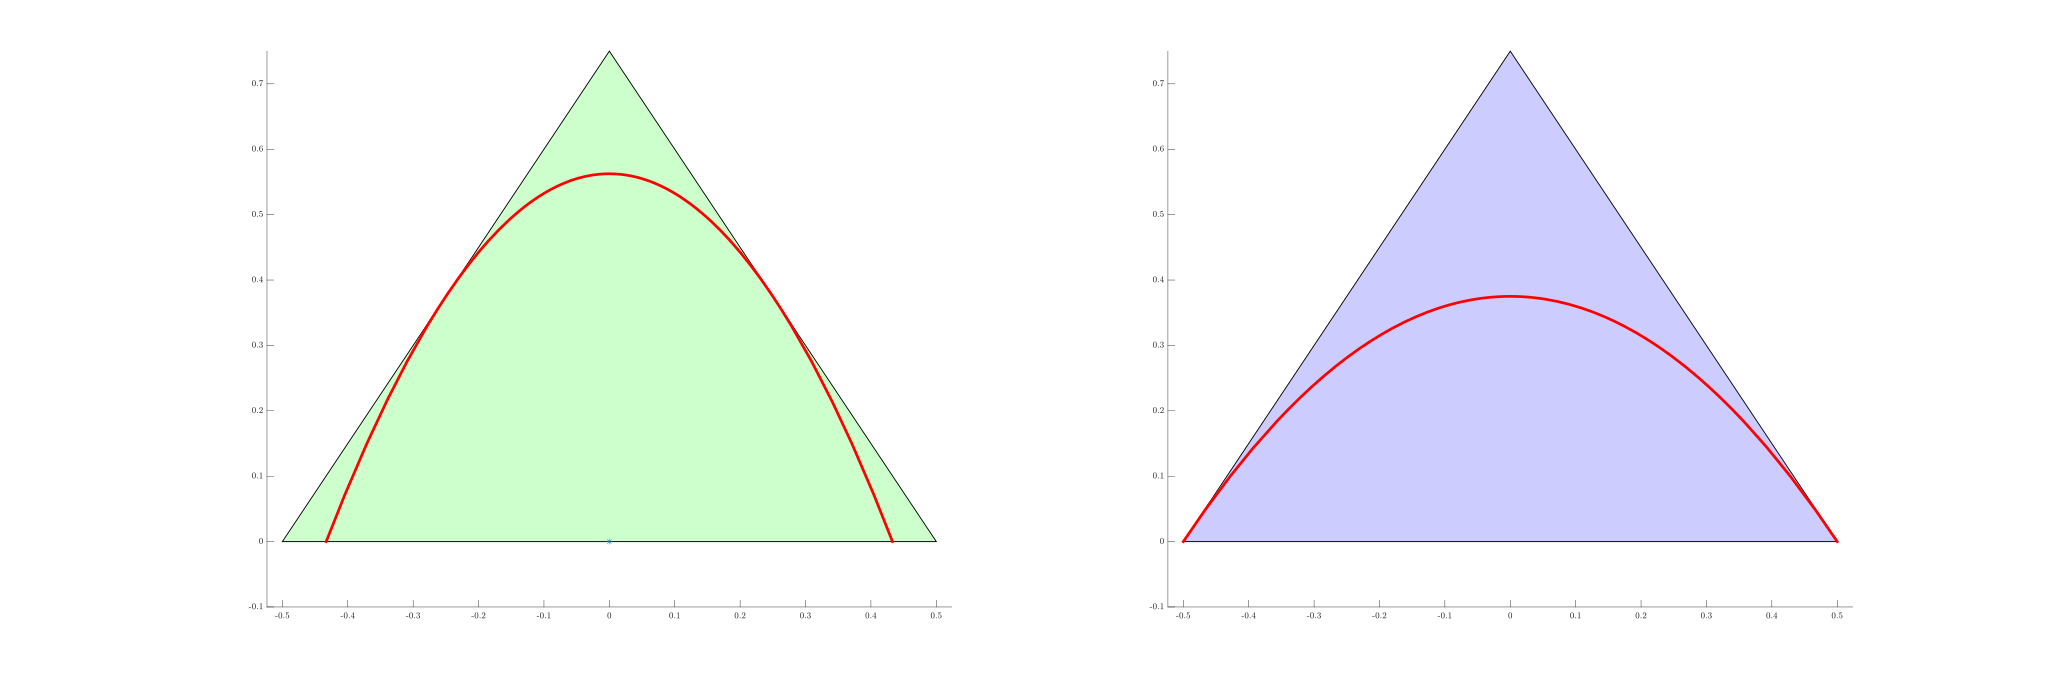
\includegraphics[width=0.8\columnwidth]{src/imgs/comparison2d_simplex_given}
\par\end{centering}
}\caption{Comparison between the MINVO, Bernstein and B-Spline bases for $n=2$.
\label{fig:Comparison2d}}
\end{figure}

{\setlength\extrarowheight{1pt}
 \setlength\tabcolsep{0pt}
%\renewcommand{\arraystretch}{1.}

\begin{table*}
\noindent\resizebox{\textwidth}{!}{%
\begin{centering}
\begin{tabular}{|c|c|c|c|c|>{\columncolor{problem3_color}\centering}c|>{\columncolor{problem4_color}\centering}c|}
\hline 
\textbf{\hspace{0.1cm}$\boldsymbol{n}$} & $\boldsymbol{A}_{\text{MV}}$ & $abs\left(\left|\boldsymbol{A}_{\text{MV}}\right|\right)$ & $\frac{abs\left(|\boldsymbol{A}_{\text{MV}}|\right)}{abs\left(|\boldsymbol{A}_{\text{Be}}|\right)}$ & $\frac{abs\left(|\boldsymbol{A}_{\text{MV}}|\right)}{abs\left(|\boldsymbol{A}_{\text{BS}}|\right)}$ & \textbf{Problem 3} & \textbf{Problem 4}\tabularnewline
\hline 
\hline 
$1$ & {\scriptsize{}$\frac{1}{2}\left[\begin{array}{cc}
-1 & 1\\
1 & 1
\end{array}\right]$} & $\frac{1}{2}=0.5$ & $=1$ & $=1$ & Global Opt. & Global Opt.\tabularnewline
\hline 
$2$ & {\scriptsize{}$\frac{1}{8}\left[\begin{array}{ccc}
3 & -2\sqrt{3} & 1\\
-6 & 0 & 6\\
3 & 2\sqrt{3} & 1
\end{array}\right]$} & $\frac{3\sqrt{3}}{16}\approx0.3248$ & $\approx1.299$ & $\approx5.196$ & Global Opt. & Global Opt.\tabularnewline
\hline 
$3$ & {\scriptsize{}$\left[\begin{array}{cccc}
-0.4302 & 0.4568 & -0.02698 & 0.0004103\\
0.8349 & -0.4568 & -0.7921 & 0.4996\\
-0.8349 & -0.4568 & 0.7921 & 0.4996\\
0.4302 & 0.4568 & 0.02698 & 0.0004103
\end{array}\right]$} & $\approx0.3319$ & $\approx2.360$ & $\approx254.9$ & Global Opt. & Global Opt.\tabularnewline
\hline 
$4$ & {\scriptsize{}$\left[\begin{array}{ccccc}
0.5255 & -0.5758 & -0.09435 & 0.1381 & 0.03023\\
-1.108 & 0.8108 & 0.9602 & -0.8108 & 0.1483\\
1.166 & 0 & -1.732 & 0 & 0.643\\
-1.108 & -0.8108 & 0.9602 & 0.8108 & 0.1483\\
0.5255 & 0.5758 & -0.09435 & -0.1381 & 0.03023
\end{array}\right]$} & $\approx0.5678$ & $\approx6.057$ & $\approx1.675\cdot10^{5}$ & $\begin{array}{c}
\text{Local Opt.}\\
\text{(at least)}
\end{array}$ & $\begin{array}{c}
\text{Local Opt.}\\
\text{(at least)}
\end{array}$\tabularnewline
\hline 
$5$ & {\scriptsize{}$\left[\begin{array}{cccccc}
-0.7392 & 0.7769 & 0.3302 & -0.3773 & -0.0365 & 0.04589\\
1.503 & -1.319 & -1.366 & 1.333 & -0.121 & 0.002895\\
-1.75 & 0.5424 & 2.777 & -0.9557 & -1.064 & 0.4512\\
1.75 & 0.5424 & -2.777 & -0.9557 & 1.064 & 0.4512\\
-1.503 & -1.319 & 1.366 & 1.333 & 0.121 & 0.002895\\
0.7392 & 0.7769 & -0.3302 & -0.3773 & 0.0365 & 0.04589
\end{array}\right]$} & $\approx1.6987$ & $\approx22.27$ & $\approx1.924\cdot10^{9}$ & $\begin{array}{c}
\text{Feasible}\\
\text{(at least)}
\end{array}$ & $\begin{array}{c}
\text{Local Opt.}\\
\text{(at least)}
\end{array}$\tabularnewline
\hline 
$6$ & {\scriptsize{}$\left[\begin{array}{ccccccc}
1.06 & -1.134 & -0.7357 & 0.8348 & 0.1053 & -0.1368 & 0.01836\\
-2.227 & 2.055 & 2.281 & -2.299 & -0.08426 & 0.2433 & 0.0312\\
2.59 & -1.408 & -4.27 & 2.468 & 1.58 & -1.081 & 0.152\\
-2.844 & 0 & 5.45 & 0 & -3.203 & 0 & 0.5969\\
2.59 & 1.408 & -4.27 & -2.468 & 1.58 & 1.081 & 0.152\\
-2.227 & -2.055 & 2.281 & 2.299 & -0.08426 & -0.2433 & 0.0312\\
1.06 & 1.134 & -0.7357 & -0.8348 & 0.1053 & 0.1368 & 0.01836
\end{array}\right]$} & $\approx9.1027$ & $\approx117.8$ & $\approx4.750\cdot10^{14}$ & $\begin{array}{c}
\text{Feasible}\\
\text{(at least)}
\end{array}$ & $\begin{array}{c}
\text{Local Opt.}\\
\text{(at least)}
\end{array}$\tabularnewline
\hline 
$7$ & {\scriptsize{}$\left[\begin{array}{cccccccc}
-1.637 & 1.707 & 1.563 & -1.682 & -0.3586 & 0.4143 & -0.006851 & 2.854\cdot10^{-5}\\
3.343 & -3.285 & -3.947 & 4.173 & 0.6343 & -0.9385 & -0.02111 & 0.05961\\
-4.053 & 2.722 & 6.935 & -4.96 & -2.706 & 2.269 & -0.2129 & 0.00535\\
4.478 & -1.144 & -9.462 & 2.469 & 6.311 & -1.745 & -1.312 & 0.435\\
-4.478 & -1.144 & 9.462 & 2.469 & -6.311 & -1.745 & 1.312 & 0.435\\
4.053 & 2.722 & -6.935 & -4.96 & 2.706 & 2.269 & 0.2129 & 0.00535\\
-3.343 & -3.285 & 3.947 & 4.173 & -0.6343 & -0.9385 & 0.02111 & 0.05961\\
1.637 & 1.707 & -1.563 & -1.682 & 0.3586 & 0.4143 & 0.006851 & 2.854\cdot10^{-5}
\end{array}\right]$} & $\approx89.0191$ & $\approx902.7$ & $\approx2.997\cdot10^{21}$ & $\begin{array}{c}
\text{Feasible}\\
\text{(at least)}
\end{array}$ & $\begin{array}{c}
\text{Local Opt.}\\
\text{(at least)}
\end{array}$\tabularnewline
\hline 
\end{tabular}
\par\end{centering}
}

\caption{Results for the MINVO basis. $\boldsymbol{A}_{\text{MV}}$, $\boldsymbol{A}_{\text{Be}}$
and $\boldsymbol{A}_{\text{BS}}$ denote the coefficient matrix of
the MINVO, Bernstein and B-Spline bases respectively ($t\in[-1,1]$).
The bigger the absolute value of the determinant, the smaller the
associated simplex (for Problem 1) and the bigger the convex hull
of the curve (for Problem 2). The matrices $\boldsymbol{A}_{\text{MV}}$
found are independent of the polynomial curve given (in Problem 1),
or of the simplex given (in Problem 2). \label{tab:table_matrices}}
\end{table*}

}

\begin{figure*}
\begin{centering}
\includegraphics[width=1\textwidth]{src/imgs/plots_basis}
\par\end{centering}
\caption{Comparison between the MINVO, Bernstein, B-Spline, and Lagrange bases
for $n=1:7$. All these bases satisfy $\sum_{i=0}^{n}\lambda_{i}(t)=1$,
and the MINVO, Bernstein and B-Spline bases also satisfy $\lambda_{i}(t)\ge0\;\;\forall t\in[-1,1]$
\label{fig:minvo_and_bernstein}}

\vskip-2ex
\end{figure*}

{\setlength\extrarowheight{1pt}
 \setlength\tabcolsep{0pt}
%\renewcommand{\arraystretch}{1.}

\begin{table}
%\noindent\resizebox{0.8\columnwidth}{!}{%
\centering
\begin{centering}
\begin{tabular}{|c|l|}
\hline 
\textbf{\hspace{0.1cm}$\boldsymbol{n}$\hspace{0.1cm}} & \qquad{}\qquad{}\qquad{}\qquad{}Roots of $\lambda_{i}(t),\;t\in[-1,1]$\tabularnewline
\hline 
\hline 
$1$ & {\scriptsize{}$\left[\begin{array}{c}
\boldsymbol{r}(\lambda_{0})^{T}\\
\boldsymbol{r}(\lambda_{1})^{T}
\end{array}\right]=\left[\begin{array}{c}
1.0\\
-1.0
\end{array}\right]$}\tabularnewline
\hline 
$2$ & {\scriptsize{}$\left[\begin{array}{c}
\boldsymbol{r}(\lambda_{0})^{T}\\
\boldsymbol{r}(\lambda_{1})^{T}\\
\boldsymbol{r}(\lambda_{2})^{T}
\end{array}\right]=\left[\begin{array}{cc}
0.5774 & \mathrm{}\\
-1.0 & 1.0\\
-0.5774 & \mathrm{}
\end{array}\right]$}\tabularnewline
\hline 
$3$ & {\scriptsize{}$\left[\begin{array}{c}
\boldsymbol{r}(\lambda_{0})^{T}\\
\boldsymbol{r}(\lambda_{1})^{T}\\
\boldsymbol{r}(\lambda_{2})^{T}\\
\boldsymbol{r}(\lambda_{3})^{T}
\end{array}\right]=\left[\begin{array}{cc}
0.03088 & 1.0\\
-1.0 & 0.7735\\
-0.7735 & 1.0\\
-1.0 & -0.03088
\end{array}\right]$}\tabularnewline
\hline 
$4$ & {\scriptsize{}$\left[\begin{array}{c}
\boldsymbol{r}(\lambda_{0})^{T}\\
\boldsymbol{r}(\lambda_{1})^{T}\\
\boldsymbol{r}(\lambda_{2})^{T}\\
\boldsymbol{r}(\lambda_{3})^{T}\\
\boldsymbol{r}(\lambda_{4})^{T}
\end{array}\right]=\left[\begin{array}{ccc}
-0.2872 & 0.835 & \mathrm{}\\
-1.0 & 0.3657 & 1.0\\
-0.8618 & 0.8618 & \mathrm{}\\
-1.0 & -0.3657 & 1.0\\
-0.835 & 0.2872
\end{array}\right]$}\tabularnewline
\hline 
$5$ & {\scriptsize{}$\left[\begin{array}{c}
\boldsymbol{r}(\lambda_{0})^{T}\\
\boldsymbol{r}(\lambda_{1})^{T}\\
\boldsymbol{r}(\lambda_{2})^{T}\\
\boldsymbol{r}(\lambda_{3})^{T}\\
\boldsymbol{r}(\lambda_{4})^{T}\\
\boldsymbol{r}(\lambda_{5})^{T}
\end{array}\right]=\left[\begin{array}{ccc}
-0.4866 & 0.5121 & 1.0\\
-1.0 & 0.04934 & 0.8895\\
-0.9057 & 0.5606 & 1.0\\
-1.0 & -0.5606 & 0.9057\\
-0.8895 & -0.04934 & 1.0\\
-1.0 & -0.5121 & 0.4866
\end{array}\right]$}\tabularnewline
\hline 
$6$ & {\scriptsize{}$\left[\begin{array}{c}
\boldsymbol{r}(\lambda_{0})^{T}\\
\boldsymbol{r}(\lambda_{1})^{T}\\
\boldsymbol{r}(\lambda_{2})^{T}\\
\boldsymbol{r}(\lambda_{3})^{T}\\
\boldsymbol{r}(\lambda_{4})^{T}\\
\boldsymbol{r}(\lambda_{5})^{T}\\
\boldsymbol{r}(\lambda_{6})^{T}
\end{array}\right]=\left[\begin{array}{cccc}
-0.6135 & 0.2348 & 0.9137 & \mathrm{}\\
-1.0 & -0.1835 & 0.6449 & 1.0\\
-0.9317 & 0.2822 & 0.9214 & \mathrm{}\\
-1.0 & -0.6768 & 0.6768 & 1.0\\
-0.9214 & -0.2822 & 0.9317 & \mathrm{}\\
-1.0 & -0.6449 & 0.1835 & 1.0\\
-0.9137 & -0.2348 & 0.6135 & \mathrm{}
\end{array}\right]$}\tabularnewline
\hline 
$7$ & {\scriptsize{}$\left[\begin{array}{c}
\boldsymbol{r}(\lambda_{0})^{T}\\
\boldsymbol{r}(\lambda_{1})^{T}\\
\boldsymbol{r}(\lambda_{2})^{T}\\
\boldsymbol{r}(\lambda_{3})^{T}\\
\boldsymbol{r}(\lambda_{4})^{T}\\
\boldsymbol{r}(\lambda_{5})^{T}\\
\boldsymbol{r}(\lambda_{6})^{T}\\
\boldsymbol{r}(\lambda_{7})^{T}
\end{array}\right]=\left[\begin{array}{cccc}
-0.7 & 0.008364 & 0.7132 & 1.0\\
-1.0 & -0.3509 & 0.4068 & 0.9355\\
-0.9481 & 0.05239 & 0.7315 & 1.0\\
-1.0 & -0.753 & 0.4399 & 0.9408\\
-0.9408 & -0.4399 & 0.753 & 1.0\\
-1.0 & -0.7315 & -0.05239 & 0.9481\\
-0.9355 & -0.4068 & 0.3509 & 1.0\\
-1.0 & -0.7132 & -0.008364 & 0.7
\end{array}\right]$}\tabularnewline
\hline 
\end{tabular}
\par\end{centering}
%}

\caption{Roots of each $\lambda_{i}(t)$. $\boldsymbol{r}(\lambda_{i}(t))$
is the column vector that contains the roots of $\lambda_{i}(t)$.
All the roots $\in(-1,1)$ are double roots. The roots $\in\{-1,1\}$
are single roots. Each $\lambda_{i}(t)$ has $n$ real roots in total.
\label{tab:roots}}
\end{table}

}

\begin{figure}
\begin{centering}
\subfloat[Simplexes found by the MINVO basis for 4 different $3^{rd}$-degree
polynomials given (Problem 1). \label{fig:Comparison3d_poly_given-1}]{\centering{}\includegraphics[width=1\columnwidth]{src/imgs/many_comparisons3d_poly_given}}
\par\end{centering}
\subfloat[Polynomial curves obtained using the MINVO basis for 4 different given
simplexes (Problem 2) \label{fig:Comparison3d_simplex_given-1}]{\begin{centering}
\includegraphics[width=1\columnwidth]{src/imgs/many_comparisons3d_simplex_given_compressed2}
\par\end{centering}
}\caption{MINVO results for $n=3$, where global optimality is guaranteed\label{fig:Comparison3d-1}}
\end{figure}

When the polynomial curve is given (i.e. Problem 1), the ratio between
the volume of the simplex $S_{\alpha}$ obtained by a basis $\alpha$
and the volume of the simplex $S_{\beta}$ obtained by a basis $\beta$
($\alpha,\beta\in{\text{MV},\text{Be},\text{BS}}$) is given by

\[
\frac{\text{vol}\left(S_{\alpha}\right)}{\text{vol}\left(S_{\beta}\right)}=\frac{\text{abs}\left(|\boldsymbol{A}_{\beta}|\right)}{\text{abs}\left(|\boldsymbol{A}_{\alpha}|\right)}
\]

Similarly, when the simplex is given (i.e. Problem 2), the ratio between
the volume of the convex hull of the polynomial curve $\boldsymbol{p}_{\alpha}(t)$
found by a basis $\alpha$ and the volume of the convex hull of the
polynomial curve $\boldsymbol{p}_{\beta}(t)$ found by a basis $\beta$
($\alpha,\beta\in{\text{MV},\text{Be},\text{BS}}$) is given by

\[
\frac{\text{vol}\left(\text{conv}\left(\boldsymbol{p}_{\alpha}(t)\right)\right)}{\text{vol}\left(\text{conv}\left(\boldsymbol{p}_{\beta}(t)\right)\right)}=\frac{\text{abs}\left(|\boldsymbol{A}_{\alpha}|\right)}{\text{abs}\left(|\boldsymbol{A}_{\beta}|\right)}
\]

These ratios are shown in Table \ref{tab:table_matrices}. The ratios
obtained mean the following for Problem 1 (Problem 2 respectively):
\begin{itemize}
\item For $n=3$, the MINVO basis finds a simplex that has a volume (a polynomial
curve whose convex hull has a volume) $\approx2.36$ and $\approx254.9$
times smaller (bigger) than the one the Bernstein and B-Spline bases
find respectively. 
\item For $n=7$, the MINVO basis finds a simplex that has a volume (a polynomial
curve whose convex hull has a volume)$\approx902.7$ and $\approx2.997\cdot10^{21}$
times smaller (bigger) than the one the Bernstein and B-Spline bases
find respectively. 
\end{itemize}
And same applies for other $n$. These comparison are shown in Fig.
\ref{fig:Comparison2d} (for $n=2$), and in Fig. \ref{fig:Comparison3d}
(for $n=3$). 

\section{Conversion between MINVO, Bernstein/B�zier and B-Spline}

Given an $n$-th order polynomial curve $\boldsymbol{p}(t)=:\boldsymbol{P}\boldsymbol{t}$,
the MINVO, B�zier or B-Spline control points (i.e. the vertexes of
the simplex that enclose that curve) can be obtained using the formula
\[
\boldsymbol{V}_{x}=\boldsymbol{P}\left(\boldsymbol{A}_{x}\right)^{-1}=\boldsymbol{V}_{y}\boldsymbol{A}_{y}\left(\boldsymbol{A}_{x}\right)^{-1}
\]

where $x,y\in\{\text{MV},\text{Be},\text{BS}\}$ (MINVO, Bernstein,
B-Spline respectively). For instance to convert from MINVO control
points to Bernstein control points we have that $\boldsymbol{V}_{\text{Be}}=\boldsymbol{P}\left(\boldsymbol{A}_{\text{Be}}\right)^{-1}=\boldsymbol{V}_{\text{MV}}\boldsymbol{A}_{\text{MV}}\left(\boldsymbol{A}_{\text{Be}}\right)^{-1}$.
The matrices $\boldsymbol{A}_{\text{MV}}$ are the ones shown in table
\ref{tab:table_matrices}, while the matrices $\boldsymbol{A}_{\text{BS}}$
and $\boldsymbol{A}_{\text{Be}}$ are available in \cite{qin2000general}.
Note that all the matrices need to be expressed in the same interval
($t\in[-1,1]$ in this paper). The code provided with this paper contains
functions that generate all these matrices. 

\textcolor{red}{==}

\textcolor{red}{Note that all the solutions found satisfy the neccesary
condition found by \cite{klee1986facet} (the centroid of each face
belongs to the convex body. In our case, to the convex hull of the
curve)}

\textcolor{red}{Citar \cite{kuti2014minimal} (obtains same result
for $n=2$)}

\textcolor{red}{Authors name stackoverflow references?}

\section{Curve contained in a subspace $\mathbb{R}^{n}\subseteq\mathbb{R}^{k}$\label{sec:Embedding}}

So far we have studied the case of $n=m=k$ (i.e. a polynomial curve
of degree $n$ and dimension $k=n$ and for which the $n$ is also
smallest dimension of the subpsace the curve is contained in, see
Sec. \ref{sec:Notation-and-Definitions}) . The case $n=m<k$ can
easily be solved by simply doing a change of basis between $\mathbb{R}^{n}$
and $\mathbb{R}^{k}$. Defining $\boldsymbol{T}_{k\times n}$ as the
transformation matrix that takes one point $\boldsymbol{a}'$ expressed
in the standard basis of $\mathbb{R}^{n}$ and transforms it to the
standard basis of $\mathbb{R}^{k}$ (i.e. $\boldsymbol{a}_{k\times1}=\boldsymbol{T}_{k\times n}\left(\boldsymbol{a}'\right)_{n\times1}$),
the following relationships hold:
\begin{center}
\begin{tabular}{|c|c|c|c|}
\hline 
 & $\mathbb{R}^{k}$ & $\mathbb{R}^{n}$ & Relationship\tabularnewline
\hline 
\hline 
Vertexes & $\boldsymbol{V}_{k\times(n+1)}$ & $\boldsymbol{V}'_{n\times(n+1)}$ & $\boldsymbol{V}=\boldsymbol{T}\boldsymbol{V}'$\tabularnewline
\hline 
Coeff. Matrix & $\boldsymbol{P}_{k\times(n+1)}$ & $\boldsymbol{P}'_{n\times(n+1)}$ & $\boldsymbol{P}=\boldsymbol{T}\boldsymbol{P}'$\tabularnewline
\hline 
\end{tabular}
\par\end{center}

Using the results for $\mathbb{R}^{n}$ (either from problem 1 or
2), we have that $\boldsymbol{P}'=\boldsymbol{V}'\boldsymbol{A}_{(n+1)\times(n+1)}^{\text{MV}}$
(where $\boldsymbol{P}'$ is given for problem 1, and and $\boldsymbol{V}'$
is given for problem 2). Therefore, we have that:

\[
\boldsymbol{P}=\boldsymbol{T}\boldsymbol{P}'=\boldsymbol{T}\boldsymbol{V}'\boldsymbol{A}_{(n+1)\times(n+1)}^{\text{MV}}=\boldsymbol{V}\boldsymbol{A}_{(n+1)\times(n+1)}^{\text{MV}}
\]

which means that, to obtain the $(n+1)$ vertexes (expressed in $\mathbb{R}^{k}$)
of the smallest $n$-simplex enclosing a polynomial curve of degree
$n$ embedded in $\mathbb{R}^{n}\subseteq\mathbb{R}^{k}$, we can
simply use:

\[
\boldsymbol{V}_{k\times(n+1)}=\boldsymbol{P}_{k\times(n+1)}\left(\boldsymbol{A}_{(n+1)\times(n+1)}^{\text{MV}}\right)^{-1}
\]

And same applies for the problem 2, but using:
\[
\boldsymbol{P}_{k\times(n+1)}=\boldsymbol{V}_{k\times(n+1)}\boldsymbol{A}_{(n+1)\times(n+1)}^{\text{MV}}
\]

For $k=3$, the cases $n=2$ and $n=1$ are shown in Fig. \ref{fig:embedding}. 

\begin{figure}
\begin{centering}
\includegraphics[width=0.9\columnwidth]{src/imgs/embedded}
\par\end{centering}
\caption{MINVO basis applied for the case $\mathbb{R}^{n}\subseteq\mathbb{R}^{k}$.
In this example we have two cases with $k=3$: On the left $n=2$
(planar curve embedded in $\mathbb{R}^{3}$), and on the right $n=1$
(segment embedded in $\mathbb{R}^{3}$) \label{fig:embedding}}

\vskip-2ex
\end{figure}


\section{Necessary condition}

As explained in Sec. \ref{sec:Introduction}, any locally optimal
simplex (with respect to its volume) must be a centroidal simplex
(i.e. the centroid of its facets must belong to $\text{conv}\left(\boldsymbol{p}(t)\right)$)
\cite{klee1986facet}. Here we prove 

\section{Conclusions and Future Work}

This work derived and presented the MINVO basis. The key features
of this basis is that it finds the smallest $n$-simplex that encloses
a given polynomial curve (Problem 1), and also finds the polynomial
curve that is inside a given simplex, and whose coefficient vectors
$\boldsymbol{p}_{n},...,\boldsymbol{p}_{1}$ span a parallelogram
with largest volume (Problem 2). Global optimality was also proven
for some $n$.

The exciting results of this work naturally lead to the following
questions and conjectures, that we leave as future work:
\begin{itemize}
\item Is the global optimum of Problem 3 the same as the global optimum
of Problem 4? In other words, are we losing optimality by imposing
the specific structure in $\lambda_{i}(t)$? The results seem to indicate
that it is likely that no optimality is lost. 
\item Does there exist an analytical solution (i.e. not numerical) for Problem
3 for any degree $n$? 
\item Does there exist a recursive formula to obtain the solution of problem
3 for $n$ given the previous solutions $1,...,n-1$? Would this recursive
formula allow to easily prove global optimality $\forall n$ of Problem
3?
\end{itemize}

\section{Acknowledgements}

The authors would like to thank Prof. Gilbert Strang, Prof. Johan
L�fberg, Ashkan M. Jasour, Kasra Khosoussi, Kaveh Fathian, Michael
Everett, Juan Jos� Madrigal and Marc Adill�n for helpul insights and
discussions.\textcolor{red}{{} Is this anonymous??}

\selectlanguage{english}%
\bibliographystyle{unsrt}
\addcontentsline{toc}{section}{\refname}\bibliography{bibliography}

\selectlanguage{american}%
\onecolumn

\section*{Appendix: Proof of Theorem 1\label{sec:Appendix}}

For this proof, we will denote $\phi_{j}(t):=t^{j}\quad\psi_{j}(t):=jt^{j-1}$
and, for $i\neq j$, define also $K_{ij}:=\int_{0}^{1}\phi_{i}(t)\psi_{j}(t)=j\int_{0}^{1}t^{i+j-1}=\frac{j}{i+j}$.
Let us also define the $(n+1)\times(n+1)$ matrix $\hat{\boldsymbol{K}}$
with zeros in the diagonal and 
\[
\hat{K}_{ij}:=\frac{1}{2}\left(K_{ij}-K_{ji}\right)=\frac{1}{2}\left(\frac{j-i}{j+i}\right)\quad i\neq j
\]

We will also define $\boldsymbol{f}(t):=\left[\begin{array}{cccc}
t^{n} & t^{n-1} & \cdots & t\end{array}\right]^{T}$.
\begin{itemize}
\item \textbf{If $n$ is odd }($n=3,5,7,...$). Let us define $a:=\frac{n+1}{2}$,
and the parameters $\alpha_{0},\alpha_{1},...,\alpha_{a-2}$  and
$t_{0},t_{1},...,t_{a-1}$ . Moreover, and unless otherwise noted,
we will use $i\in\{0,1,...,a-1\}$ and $j\in\{0,1,...,a-1\}$ Using
the corollary of \cite{mazur2017convex} \textcolor{red}{(Sec. 1)},
every point in $\text{conv}(\boldsymbol{p}(t))$ can be expressed
as a convex combination of $a$ points of the polynomial curve. (This
paper provides, for a polynomial curve, a tighter bound than \cite{eckhoff1993helly}.
Denote these points as $\boldsymbol{p}(t_{0}),...,\boldsymbol{p}(t_{a-1})$.
We have then that: \textcolor{red}{Check that I only need this amount
of points. }

\[
\boldsymbol{p}(t)=\alpha_{0}\boldsymbol{p}(t_{0})+...+\alpha_{a-2}\boldsymbol{p}(t_{a-2})+\left(1-\sum_{i=0}^{a-2}\alpha_{i}\right)\boldsymbol{p}(t_{a-1})\quad\alpha_{i+1}>\alpha_{i},0,1-\sum_{i=0}^{a-2}\alpha_{i}>0,t_{i}\in[0,1],t_{i}>t_{i-1}
\]

And therefore, the volume is given by:

\[
\text{vol}\left(\text{conv}\left(\boldsymbol{p}(t)\right)\right)=\overbrace{\int_{0}^{1}\int_{0}^{1-\alpha_{0}}\int_{0}^{1-\alpha_{0}-\alpha_{1}}...\int_{0}^{1-\sum_{i=0}^{a-3}\alpha_{i}}}^{a-1\text{ integrals}}\left[\overbrace{\int_{-1}^{1}\int_{t_{0}}^{1}\int_{t_{1}}^{1}...\int_{t_{a-2}}^{1}}^{a\text{ integrals}}\text{abs}\left(J\right)dt_{a-1}dt_{a-2}...dt_{0}\right]d\alpha_{a-2}d\alpha_{a-3}...d\alpha_{0}
\]

where $\text{abs}\left(J\right)$ is the absolute value of the Jacobian:
\[
\text{abs}\left(J\right)=\text{abs}\left(\left|\begin{array}{cccccc}
\frac{\partial\boldsymbol{p}(t)}{\alpha_{0}} & \cdots & \frac{\partial\boldsymbol{p}(t)}{\alpha_{a-2}} & \frac{\partial\boldsymbol{p}(t)}{t_{0}} & \cdots & \frac{\partial\boldsymbol{p}(t)}{t_{a-1}}\end{array}\right|\right)\labelrel={sp:propdet}\text{abs}\left(\left|\boldsymbol{P}_{:,0:n}\right|\left|\boldsymbol{R}\right|\left(\prod_{i=0}^{a-2}\alpha_{i}\right)\left(1-\sum_{i=0}^{a-2}\alpha_{i}\right)\right)
\]

where
\[
\boldsymbol{R}:=\left[\begin{array}{ccccccccccccc}
\boldsymbol{f}(t_{0})-\boldsymbol{f}(t_{a-1}) & \brokenvert & \boldsymbol{f}(t_{1})-\boldsymbol{f}(t_{a-1}) & \brokenvert & \cdots & \brokenvert & \boldsymbol{f}(t_{a-2})-\boldsymbol{f}(t_{a-1}) & \brokenvert & \frac{\partial\boldsymbol{f}(t_{0})}{\partial t_{0}} & \brokenvert & \cdots & \brokenvert & \frac{\partial\boldsymbol{f}(t_{a-1})}{\partial t_{a-1}}\end{array}\right]
\]

Now, note that:

\[
\text{abs}\left(\left|\boldsymbol{R}\right|\right)=\text{abs}\left(\left|\begin{array}{cc}
\boldsymbol{R} & \boldsymbol{f}(t_{a-1})\\
\boldsymbol{0}^{T} & 1
\end{array}\right|\right)=\text{abs}\left(\left|\begin{array}{cccccccc}
\boldsymbol{f}(t_{0}) & \boldsymbol{f}(t_{1}) & \cdots & \boldsymbol{f}(t_{a-2}) & \boldsymbol{f}(t_{a-1}) & \frac{\partial\boldsymbol{f}(t_{0})}{\partial t_{0}} & \cdots & \frac{\partial\boldsymbol{f}(t_{a-1})}{\partial t_{a-1}}\\
1 & 1 & \cdots & 1 & 1 & 0 & \cdots & 0
\end{array}\right|\right)=
\]

\[
=\text{abs}\left(\left|\begin{array}{ccccccc}
\boldsymbol{f}(t_{0}) & \frac{\partial\boldsymbol{f}(t_{0})}{\partial t_{0}} & \boldsymbol{f}(t_{1}) & \frac{\partial\boldsymbol{f}(t_{1})}{\partial t_{1}} & \cdots & \boldsymbol{f}(t_{a-1}) & \frac{\partial\boldsymbol{f}(t_{a-1})}{\partial t_{a-1}}\\
1 & 0 & 1 & 0 & \cdots & 1 & 0
\end{array}\right|_{\left(n+1\right)\times\left(n+1\right)}\right)\labelrel={sp:vander}\prod_{i<j}\left(t_{i}-t_{j}\right)^{4}=\prod_{i\neq j}\left(t_{i}-t_{j}\right)^{2}
\]

\textcolor{red}{Now, note that:}
\begin{itemize}
\item[$\circ$] $I_{1}:=\overbrace{\int_{0}^{1}\int_{0}^{1-\alpha_{0}}...\int_{0}^{1-\sum_{i=0}^{a-3}\alpha_{i}}}^{a-1\text{ integrals}}\left(\prod_{i=0}^{a-2}\alpha_{i}\right)\left(1-\sum_{i=0}^{a-2}\alpha_{i}\right)d\alpha_{a-2}d\alpha_{a-3}...d\alpha_{0}\labelrel={sp:I1}\frac{1}{n!}$
\item[$\circ$] $I_{2}:=\overbrace{\int_{-1}^{1}\int_{t_{0}}^{1}...\int_{t_{a-2}}^{1}}^{a\text{ integrals}}\text{abs}\left(\left|\boldsymbol{R}\right|\right)dt_{a-1}dt_{a-2}...dt_{0}\labelrel={sp:sym}\frac{1}{a!}\int_{[-1,1]^{a}}\text{abs}\left(\left|\boldsymbol{R}\right|\right)dV\labelrel={sp:changevar}\frac{2^{a(2a-1)}}{a!}\int_{[0,1]^{a}}\prod_{i\neq j}\left(q_{i}-q_{j}\right)^{2}dV$

\[
\text{abs}\left(\left|\hat{K}\right|\right)=\frac{1}{2^{n+1}}\prod_{0\le i<j\le n}\left(\frac{j-i}{j+i}\right)^{2}\implies\text{abs}\left(\text{Pf}(\hat{K})\right)=\frac{1}{2^{\frac{n+1}{2}}}\prod_{0\le i<j\le n}\left(\frac{j-i}{j+i}\right)
\]

And therefore, we have that $I_{2}=\frac{2^{a(2a-1)}}{a!}2^{a}(a!)\frac{1}{2^{a}}\prod_{0\le i<j\le n}\left(\frac{j-i}{j+i}\right)=2^{a(2a-1)}\prod_{0\le i<j\le n}\left(\frac{j-i}{j+i}\right)$.
Finally:

\[
\boxed{\text{vol}\left(\text{conv}\left(\boldsymbol{p}(t)\right)\right)=\text{abs}\left(\left|\boldsymbol{P}_{:,0:n}\right|\right)I_{1}I_{2}=\frac{\text{abs}\left(\left|\boldsymbol{P}_{:,0:n}\right|\right)}{n!}2^{\frac{n(n+1)}{2}}\prod_{0\le i<j\le n}\left(\frac{j-i}{j+i}\right)}
\]

\end{itemize}
\end{itemize}

\begin{itemize}
\item \textbf{If $n$ is even} ($n=2,4,6,...$): Let us define $a:=\frac{n}{2}-1$,
and the parameters $\alpha_{0},...,\alpha_{a}$ and $t_{0},...,t_{a}$
. Moreover, and unless otherwise noted, we will use $i\in\{0,1,...,a\}$
and $j\in\{0,1,...,a\}$. Using the corollary of \cite{mazur2017convex}(Sec.
1), every point in $\text{conv}(\boldsymbol{p}(t))$ can be expressed
as a convex combination of $a+2$ points of the polynomial curve,
with one point fixed (that we will take as $\boldsymbol{p}(1)$).
Denote these points as $\boldsymbol{p}(1),\boldsymbol{p}(t_{0}),...,\boldsymbol{p}(t_{a})$.
We have then that:

\[
\boldsymbol{p}(t)=\alpha_{0}\boldsymbol{p}(1)+\alpha_{1}\boldsymbol{p}(t_{0})+...+\alpha_{a}\boldsymbol{p}(t_{a-1})+\left(1-\sum_{i=0}^{a}\alpha_{i}\right)\boldsymbol{p}(t_{a})\quad\alpha_{i}>0,1-\sum_{i=0}^{a}\alpha_{i}>0,t_{i}\in[0,1],t_{i}>t_{i-1}
\]

And therefore, the volume is given by:

\[
\text{vol}\left(\text{conv}\left(\boldsymbol{p}(t)\right)\right)==\overbrace{\int_{0}^{1}\int_{0}^{1-\alpha_{0}}...\int_{0}^{1-\sum_{i=0}^{a-1}\alpha_{i}}}^{a+1\text{ integrals}}\left[\overbrace{\int_{-1}^{1}\int_{t_{0}}^{1}...\int_{t_{a-1}}^{1}}^{a+1\text{ integrals}}\text{abs}\left(J\right)dt_{a}dt_{a-1}...dt_{0}\right]d\alpha_{a}d\alpha_{a-1}...d\alpha_{0}
\]

where $\text{abs}\left(J\right)$ is the absolute value of the Jacobian:
\[
\text{abs}\left(J\right):=abs\left(\left|\begin{array}{cccccc}
\frac{\partial\boldsymbol{p}(t)}{\alpha_{0}} & \cdots & \frac{\partial\boldsymbol{p}(t)}{\alpha_{a}} & \frac{\partial\boldsymbol{p}(t)}{t_{0}} & \cdots & \frac{\partial\boldsymbol{p}(t)}{t_{a}}\end{array}\right|\right)\labelrel={sp:propdet2}\text{abs}\left(\left|\boldsymbol{P}_{:,0:n}\right|\left|\boldsymbol{R}\right|\left(\prod_{{\color{red}i=1}}^{a}\alpha_{i}\right)\left(1-\sum_{i=0}^{{\color{red}a-1}}\alpha_{i}\right)\right)
\]

where

\[
\boldsymbol{R}:=\left[\begin{array}{ccccccccccccc}
\boldsymbol{1}-\boldsymbol{f}(t_{a}) & \brokenvert & \boldsymbol{f}(t_{0})-\boldsymbol{f}(t_{a}) & \brokenvert & \cdots & \brokenvert & \boldsymbol{f}(t_{a-1})-\boldsymbol{f}(t_{a}) & \brokenvert & \frac{\partial\boldsymbol{f}(t_{0})}{\partial t_{0}} & \brokenvert & \cdots & \brokenvert & \frac{\partial\boldsymbol{f}(t_{a})}{\partial t_{a}}\end{array}\right]
\]

Now, note that:

\[
\text{abs}\left(\left|\boldsymbol{R}\right|\right)=\text{abs}\left(\left|\begin{array}{cc}
\boldsymbol{R} & \boldsymbol{f}(t_{a})\\
\boldsymbol{0}^{T} & 1
\end{array}\right|\right)=\text{abs}\left(\left|\begin{array}{cccccccc}
\boldsymbol{1} & \boldsymbol{f}(t_{0}) & \cdots & \boldsymbol{f}(t_{a-1}) & \boldsymbol{f}(t_{a}) & \frac{\partial\boldsymbol{f}(t_{0})}{\partial t_{0}} & \cdots & \frac{\partial\boldsymbol{f}(t_{a})}{\partial t_{a}}\\
1 & 1 & \cdots & 1 & 1 & 0 & \cdots & 0
\end{array}\right|\right)=
\]

\[
=\text{abs}\left(\left|\begin{array}{cccccc}
\boldsymbol{f}(t_{0}) & \frac{\partial\boldsymbol{f}(t_{0})}{\partial t_{0}} & \cdots & \boldsymbol{f}(t_{a}) & \frac{\partial\boldsymbol{f}(t_{a})}{\partial t_{a}} & \boldsymbol{1}\\
1 & 0 & \cdots & 1 & 0 & 1
\end{array}\right|\right)\labelrel={sp:vander2}\left(\prod_{i\neq j}\left(t_{i}-t_{j}\right)^{2}\right)\left(\prod_{i}\left(t_{i}-1\right)^{2}\right)
\]

\textcolor{red}{Now note that:}
\begin{itemize}
\item[$\circ$] $I_{1}:=\overbrace{\int_{0}^{1}\int_{0}^{1-\alpha_{0}}...\int_{0}^{1-\sum_{i=0}^{a-1}\alpha_{i}}}^{a+1\text{ integrals}}\left(\prod_{i=1}^{a}\alpha_{i}\right)\left(1-\sum_{i=0}^{{\color{red}a}}\alpha_{i}\right)d\alpha_{a}d\alpha_{a-1}...d\alpha_{0}=\frac{1}{n!}$
\item[$\circ$] $I_{2}:=\overbrace{\int_{-1}^{1}\int_{t_{0}}^{1}...\int_{t_{a-1}}^{1}}^{a+1\text{ integrals}}\text{abs}\left(\left|\boldsymbol{R}\right|\right)dt_{a}dt_{a-1}...dt_{0}\labelrel={sp:sym2}\frac{1}{(a+1)!}\int_{[-1,1]^{a+1}}\text{abs}\left(\left|\boldsymbol{R}\right|\right)dV\labelrel={sp:changevar2}\frac{2^{2a^{2}+5a+3}}{(a+1)!}\int_{[0,1]^{a+1}}\left(\prod_{i\neq j}\left(q_{i}-q_{j}\right)^{2}\right)\left(\prod_{i}\left(q_{i}-1\right)^{2}\right)dV$

where we have used the sustitution $t_{i}=2q_{i}-1$ and used the
simmetry. Now, note that:

\[
\text{Pf}(\hat{\boldsymbol{K}})\labelrel={sp:pfwithones}\text{Pf}\left(\left[\begin{array}{cc}
\hat{\boldsymbol{K}} & \boldsymbol{1}\\
\boldsymbol{-1^{T}} & 0
\end{array}\right]\right)\labelrel={sp:proppf}\frac{1}{2^{a+1}}\text{Pf}\left(\left[\begin{array}{cc}
2\hat{\boldsymbol{K}} & \boldsymbol{1}\\
\boldsymbol{-1^{T}} & 0
\end{array}\right]\right)
\]

and therefore we have that $I_{2}=\frac{2^{2a^{2}+5a+3}}{(a+1)!}2^{a+1}\left(\left(a+1\right)!\right)\text{abs}\left(\text{Pf}(\hat{\boldsymbol{K}})\right)=2^{2a^{2}+5a+3}\prod_{0\le i<j\le n}\left(\frac{j-i}{j+i}\right)$
. Finally:
\end{itemize}

\[
\boxed{\text{vol}\left(\text{conv}\left(\boldsymbol{p}(t)\right)\right)=\text{abs}\left(\left|\boldsymbol{P}_{:,0:n}\right|\right)I_{1}I_{2}=\frac{\text{abs}\left(\left|\boldsymbol{P}_{:,0:n}\right|\right)}{n!}2^{\frac{n(n+1)}{2}}\prod_{0\le i<j\le n}\left(\frac{j-i}{j+i}\right)}
\]

\hfill $\square$

\end{itemize}
\cite{de1955some}
\begin{itemize}
\item \ref{sp:propdet}, \ref{sp:propdet2}: Expressing the matrix as the
product of two matrices and applying the properties of the determinants. 
\item \ref{sp:vander}, \ref{sp:vander2}: See \cite{hou2015recursion,3743664}. 
\item \ref{sp:I1}: See ?? 
\item \ref{sp:sym}, \ref{sp:sym2}: Using simmetry. 
\item \ref{sp:changevar}, \ref{sp:changevar2}:Using the change of variables
$t_{i}=2q_{i}-1$ \cite{3754782}.
\item \ref{sp:pfwithones}: See \cite{de1955some}. 
\item \ref{sp:proppf}: Using the properties of the Pfaffian (\cite[Proposition~2.6]{austin2007pfaffian})
and wikipedia??
\end{itemize}
\uline{Remark:} When $\boldsymbol{p}(t)$ is the curve $\left[\begin{array}{cccc}
\frac{t+1}{2} & \left(\frac{t+1}{2}\right)^{2} & \cdots & \left(\frac{t+1}{2}\right)^{n}\end{array}\right]^{T}$, the formula matches with the one available in \cite[Theorem~15.2]{karlin1953geometry}\footnote{Note that \cite{karlin1953geometry} uses the convention $t\in[0,1]$
(instead of $t\in[-1,1]$) , and therefore it uses the curve $\left[\begin{array}{cccc}
t & t^{2} & \cdots & t^{n}\end{array}\right]^{T}$}. Indeed, for this curve we have:

\[
\text{abs}\left(\left|\boldsymbol{P}_{:,0:n}\right|\right)=\prod_{i=1}^{n}\frac{1}{2^{i}}=2^{\frac{-n(n+1)}{2}}
\]

Denoting now the beta function as $\text{B}(x,y)$, we have that:

\[
\text{vol}\left(\text{conv}\left(\boldsymbol{p}(t)\right)\right)=\frac{1}{n!}\prod_{0\le i<j\le n}\left(\frac{j-i}{j+i}\right)=\frac{1}{n!}\prod_{j=1}^{n}\left(\frac{j!(j-1)!}{(2j-1)!}\right)=\prod_{j=1}^{n}\left(\frac{\left((j-1)!\right)^{2}}{(2j-1)!}\right)=\prod_{j=1}^{n}\text{B}(j,j)
\]

which is the same formula as \cite[Theorem~15.2]{karlin1953geometry}.

\textcolor{red}{Cuidado, acordarse de poner valores absolutos everywhere!!}

\textcolor{red}{Citar theorem 2.2 y 2.3 de de http://citeseerx.ist.psu.edu/viewdoc/download?doi=10.1.1.973.6094\&rep=rep1\&type=pdf
(aunque ellos parece que lo cojen de Karlin/Shapley)}

\begin{center}
\par\end{center}

\begin{center}
\par\end{center}


\end{document}
